% DOCUMENT TYPE: PRESENTATION
\documentclass[12pt]{beamer}

% PACKAGES TO USE
\usepackage[utf8]{inputenc}
\usepackage[spanish]{babel}
\usepackage{lastpage}
\usepackage{subcaption}
\usepackage[export]{adjustbox}

% CONFIGURATIONS
\setbeamertemplate{footline}[frame number]

% PRESENTATION INFO
\title{Reconstrucción de Huellas Dactilares Digitales Utilizando un Modelo Generativo Adversarial Convolucional}
\author{Cristian Yesid Andrade Hernández}
\institute{Universidad de los Andes}
\date{2020}

% DOCUMENT
\begin{document}

% ==== INIT SLIDE ====
\frame[plain]{\titlepage}

% ==== SLIDE 1 ====
\begin{frame}{Introducción}

    Captura digital de impresión dactilar del dedo índice.

    \begin{figure}[h]
        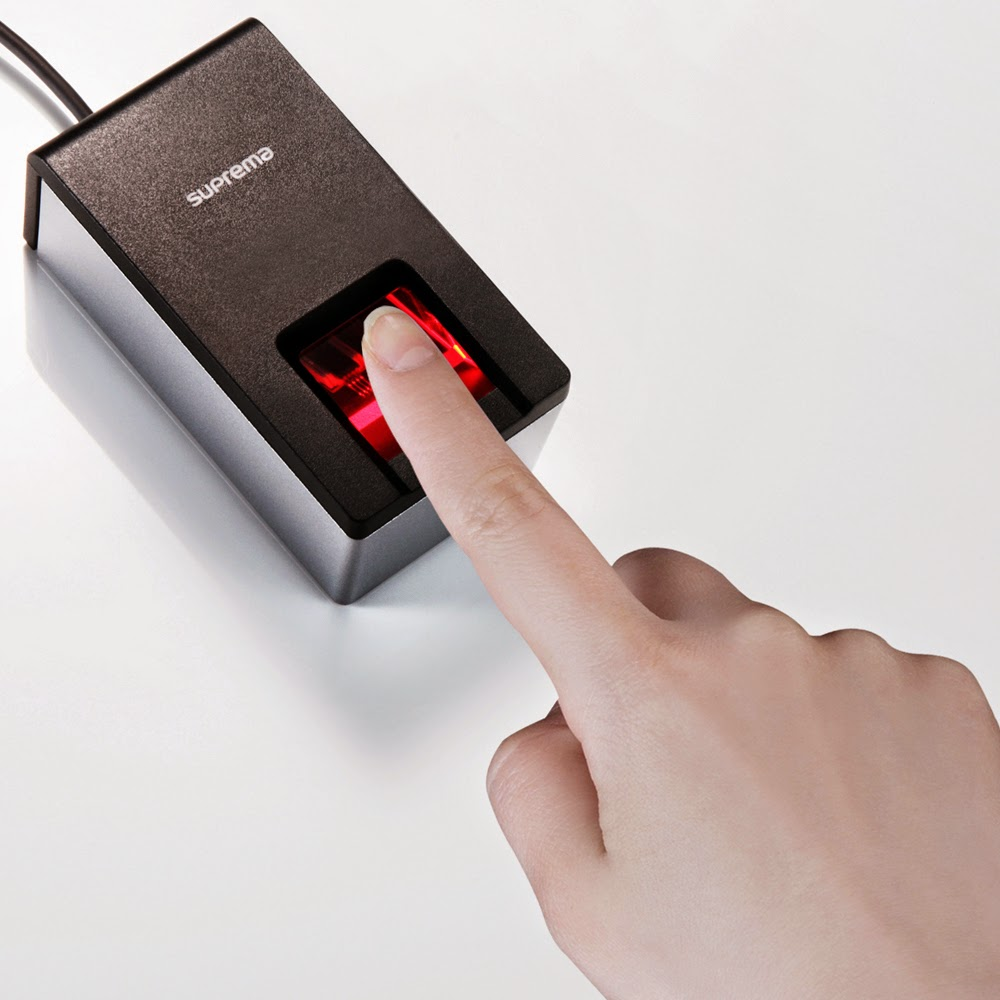
\includegraphics[scale=0.15]{figs/dedo_lector_biometrico.jpg}
        \caption{Lector Biométrico Óptico}
    \end{figure}
    
\end{frame}

% ==== SLIDE 2 ====
\begin{frame}{Introducción}

    Huellas dactilares digitalizadas con alguna condición de deterioro o modificación.
    \vspace{5mm}

    \begin{figure}[h]
        \begin{subfigure}{0.45\textwidth}
            \centering
            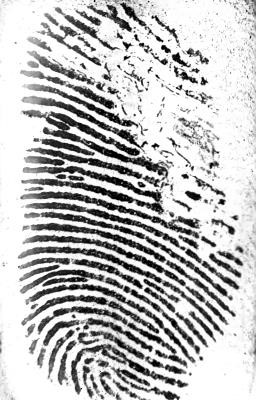
\includegraphics[scale=0.4]{figs/deteriorada_1.jpg}  
            \caption{Huella Borrosa}
        \end{subfigure}
        \begin{subfigure}{0.45\textwidth}
            \centering
            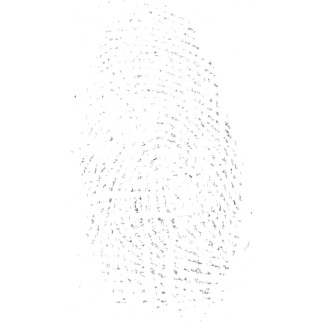
\includegraphics[scale=0.42]{figs/deteriorada_0.png}  
            \caption{Huella Incompleta}
        \end{subfigure}
    \end{figure}

\end{frame}

% ==== SLIDE 3 ====
\begin{frame}{Introducción}

    \begin{figure}[h]
        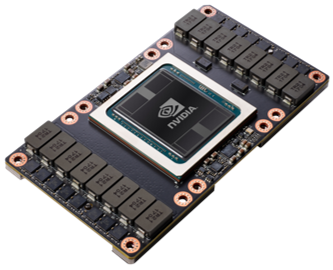
\includegraphics[scale=0.3]{figs/nvidia_card.png}
        \caption{Capacidad de Cómputo: GPU}
    \end{figure}
    
    \begin{figure}[h]
        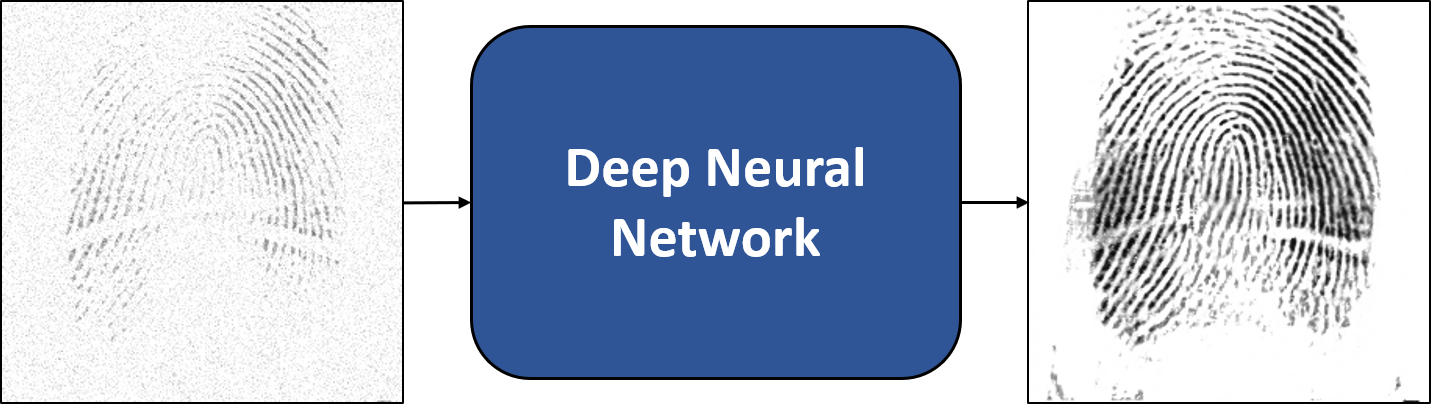
\includegraphics[scale=0.3]{figs/end_to_end.png}
        \caption{Modelo end to end}
    \end{figure}

\end{frame}

% ==== SLIDE 4 ====
\begin{frame}{Red Neuronal Convolucional}

    Composición de imagen digital de un canal.

    \begin{figure}[h]
        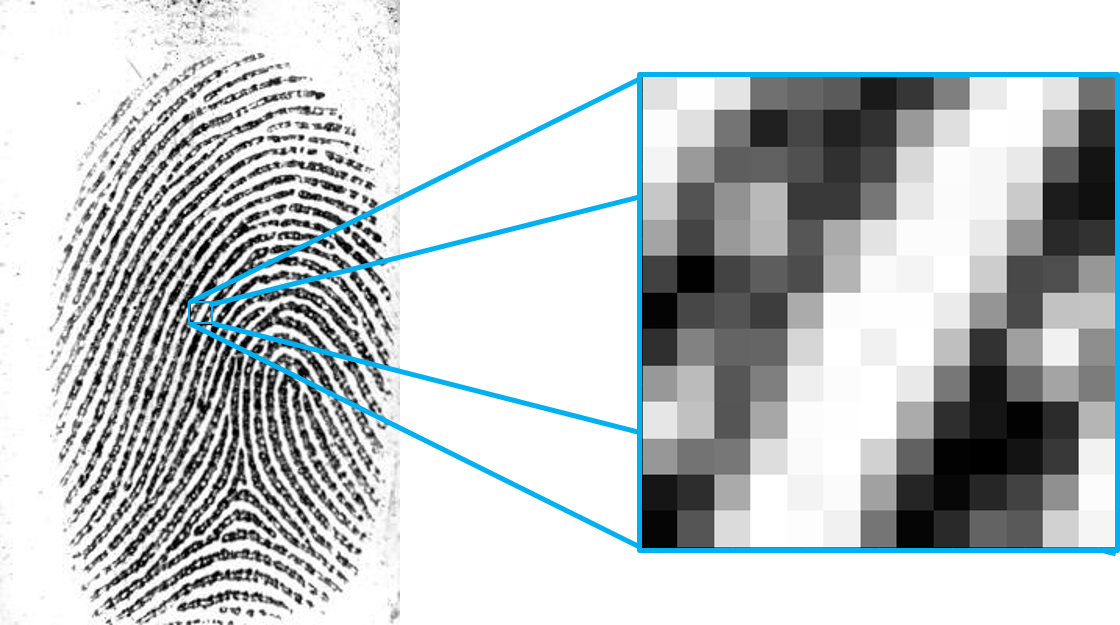
\includegraphics[scale=0.45]{figs/huella_pixeles.png}
        \caption{Huella Dactilar Digital}
    \end{figure}

\end{frame}

% ==== SLIDE 5 ====
\begin{frame}{Red Neuronal Convolucional}

    Lógica de la operación de convolución y convolución transpuesta en dos dimensiones aplicada a una imagen.

    \begin{figure}[h]
        \begin{subfigure}{0.45\textwidth}
            \centering
            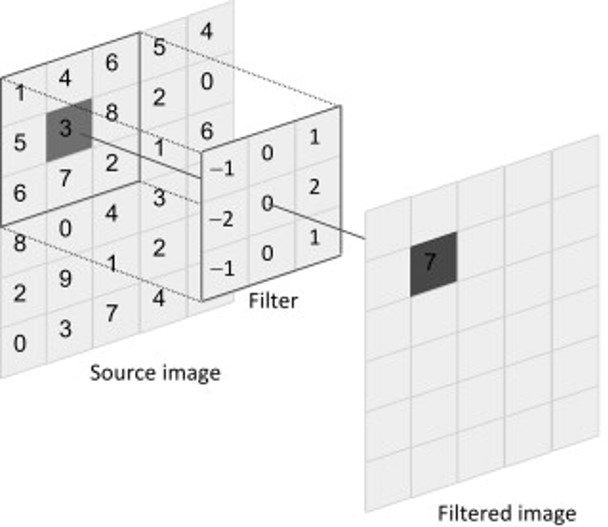
\includegraphics[scale=0.325]{figs/conv_2d.jpg}  
            \caption{Convolución}
        \end{subfigure}
        \begin{subfigure}{0.45\textwidth}
            \centering
            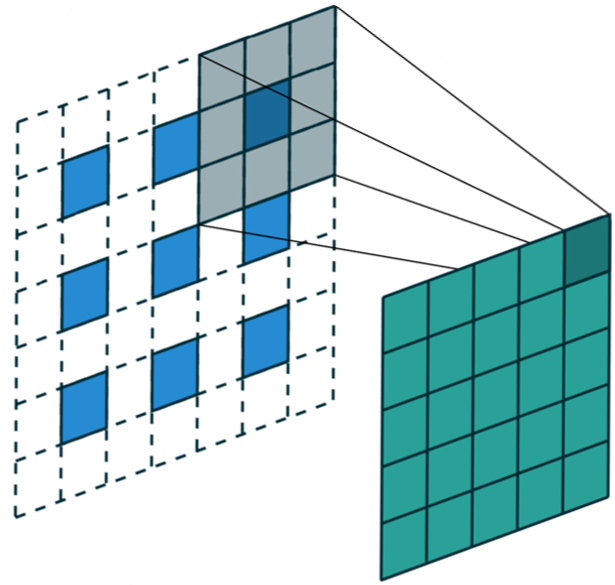
\includegraphics[scale=0.30]{figs/trans_conv.PNG}  
            \caption{Convolución Transpuesta}
        \end{subfigure}
    \end{figure}

\end{frame}

% ==== SLIDE 6 ====
\begin{frame}{Red Neuronal Convolucional}

    Modelo convolucional de reconstrucción y mejora de impresiones dactilares digitales.

    \begin{figure}[h]
        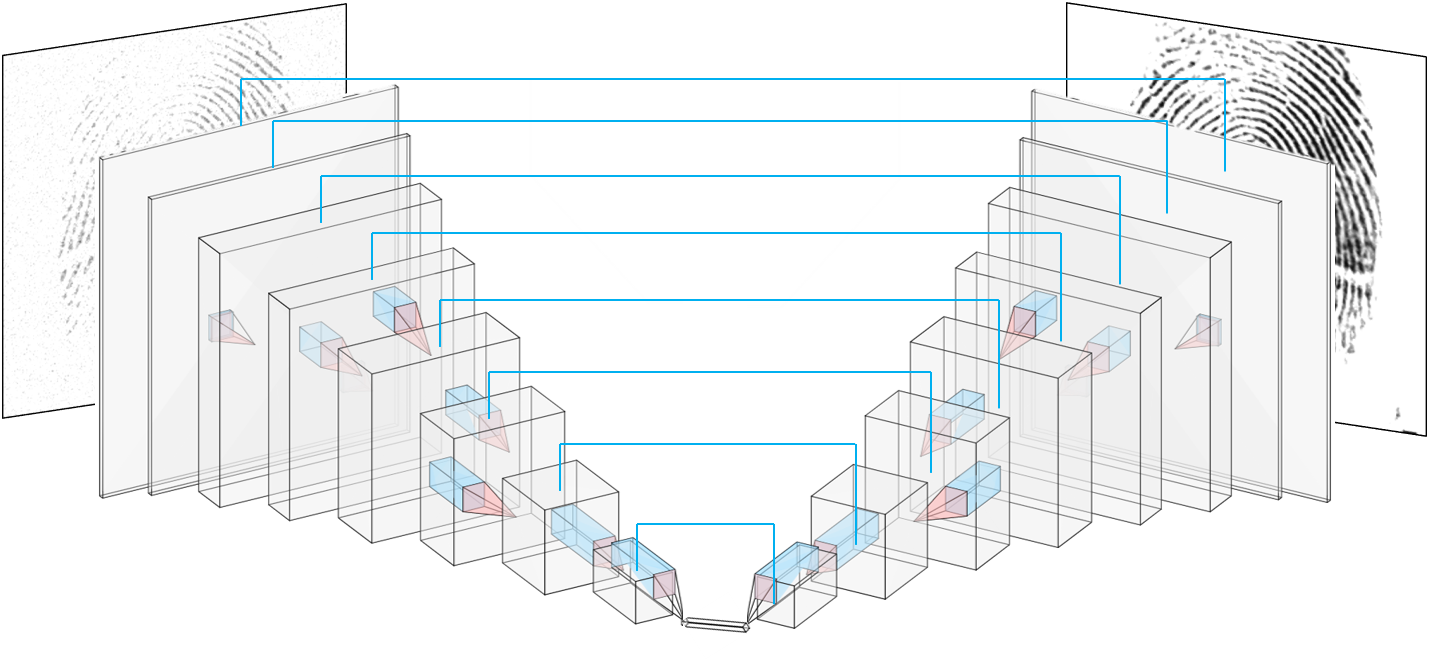
\includegraphics[scale=0.42]{figs/layers_nn_u.PNG}
        \caption{Autoencoder en Configuración U-Net}
    \end{figure}

\end{frame}

% ==== SLIDE 7 ====
\begin{frame}{Red Neuronal Convolucional}

    Ventajas de usar un modelo de capas convolucionales:
    \vspace{5mm}
    
    \begin{itemize}
        \item Características de bajo y alto nivel que se utilizan en la reconstrucción.
        \vspace{4mm}
        
        \begin{figure}[h]
            \begin{subfigure}{0.18\textwidth}
                \centering
                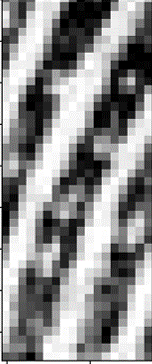
\includegraphics[scale=0.16]{figs/fll_0.png}  
                \caption{Cresta Vertical}
            \end{subfigure}
            \begin{subfigure}{0.18\textwidth}
                \centering
                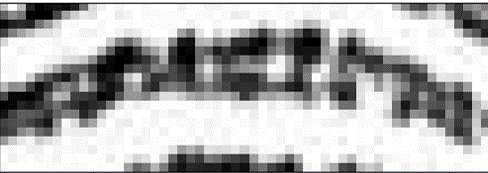
\includegraphics[scale=0.16]{figs/fll_1.png}  
                \caption{Cresta Horizontal}
            \end{subfigure}
            \begin{subfigure}{0.18\textwidth}
                \centering
                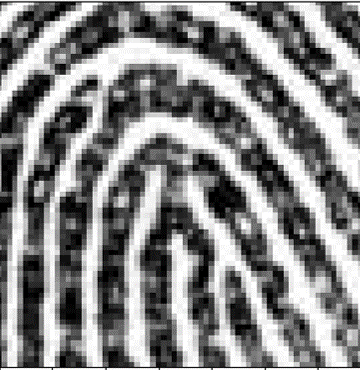
\includegraphics[scale=0.16]{figs/fhl_0.png}  
                \caption{Núcleo}
            \end{subfigure}
            \begin{subfigure}{0.18\textwidth}
                \centering
                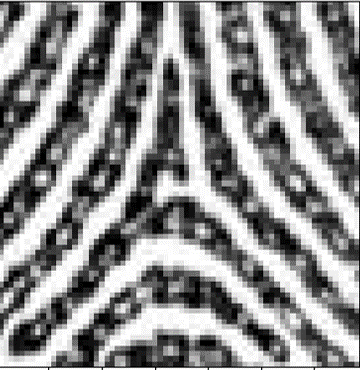
\includegraphics[scale=0.16]{figs/fhl_1.png}  
                \caption{Delta}
            \end{subfigure}
        \end{figure}
        
        \vspace{3mm}
        
        \item Modelo convolucional: 15 millones de parámetros. Perceptrón multicapa: 1000 millones de parámetros
        
    \end{itemize}

\end{frame}

\end{document}


%command	8pt	9pt	10pt	11pt	12pt	14pt	17pt	20pt
%tiny	5pt	5pt	5pt	6pt	6pt	6pt	8pt	10pt
%scriptsize	5pt	6pt	7pt	8pt	8pt	8pt	10pt	12pt
%footnotesize	6pt	7pt	8pt	9pt	10pt	10pt	12pt	14pt
%small	7pt	8pt	9pt	10pt	11pt	12pt	14pt	17pt
%normalsize	8pt	9pt	10pt	11pt	12pt	14pt	17pt	20pt
%large	10pt	10pt	12pt	12pt	14pt	17pt	20pt	25pt
%Large	11pt	11pt	14pt	14pt	17pt	20pt	25pt	29.86pt
%LARGE	12pt	12pt	17pt	17pt	20pt	25pt	29.86pt	35.83pt
%huge	14pt	14pt	20pt	20pt	25pt	29.86pt	35.83pt	42.99pt
%Huge	17pt	17pt	25pt	25pt	25pt	35.83pt	42.99pt	51.59pt